\chapter{实验}
\label{cha:method}

% 实验旨在回答以下研究问题:
% \begin{itemize}
%     \item 能否发现预测的有用语义,以进行有效得引导策略的更新?
%     \item 发现的预测语义是什么? 
%     \item 发现预测的语义有多重要? 
% \end{itemize}

\section{实验配置}
\subsection{训练环境}
为了验证本文所提出方法的有效性,本文利用 Bsuite \cite{osbandBehaviourSuiteReinforcement2019} 强化学习工具套件,实现了文献[10]附录中设计的表格型网格世界环境。如\autoref{fig:simple-gridworld}所示,彩色的小块是智能体可以收集的对象。这些对象带有不同的分数,作为智能体采取动作后的收益,有正有负。表格网格世界的对象位置是固定的,但是不同对象在被智能体收集后,得到的收益不一样,重复出现的概率不一样,同时,有的对象还可能以指定的概率使得智能体交互的情节(episode)提前终止。这样的环境虽然简单,但可以包括强化学习的基本挑战,例如延迟奖励,干扰奖励和不完全状态观察等。这样的训练环境是表格形式的,没有涉及任何函数逼近器。

在元训练的时候,采样得到的表格网格世界环境的对象的位置是不同的,但在它的生命周期里,对象的位置是固定的。而且智能体更新的时候是利用相同的环境进行调整$\theta$的值。

\begin{figure}[h!] % image examples & compare
    \begin{subfigure}{0.48\textwidth}
        \centering
        % \makebox[0.10\textwidth]{\scriptsize }\\
        \includegraphics[width=0.65\textwidth]{image/chap04/simple_grid_world.pdf}
        \caption{网格世界}
        \label{fig:simple-gridworld}
    \end{subfigure}
    \begin{subfigure}{0.48\textwidth}
        \centering
        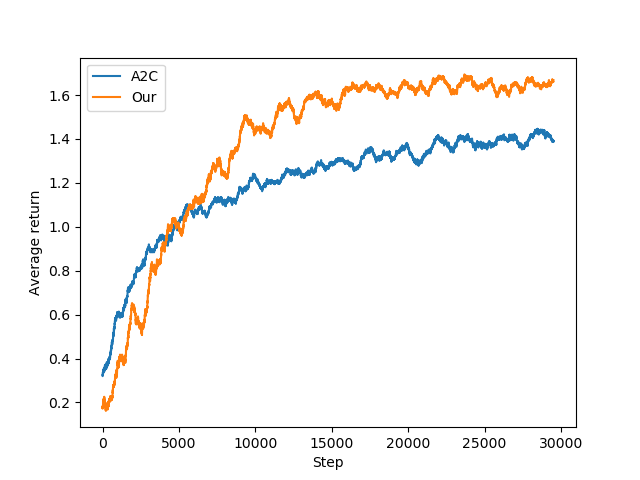
\includegraphics[width=0.88\textwidth]{image/chap04/simple.png}
        \caption{实验结果}
        \label{fig:simple-result}
    \end{subfigure}
    \caption{简单的网格世界及其实验结果}
    \label{fig:simple}
\end{figure}


\subsection{实现细节}

本文使用了20维预测向量$y \in \mathcal{R}^{20}$。 在元训练期间,本实验在智能体每交互20步更新一次智能体参数,前面所提到的A2C算法在交互没有停止的时候也是利用20步A2C算法。由于大多数情况训练的情节跨越20-2000步,因此元学习必须为预测向量$y$发现长期语义,以便能够最大化来自部分轨迹的长期未来回报。LSTM使用的是两层的多层感知机(MLP)。该算法是使用深度学习框架 pytorch \cite{paszkePytorchImperativeStyle2019} 以及Bsuite的相关工具实现的。

\section{实验结果}
在对不同环境进行元训练前,先对一个简单的网格世界重复进行元训练,然后在它上面进行智能体策略更新,其结果如\autoref{fig:simple-result}所示。其中的20维的预测向量在最后的取值 \autoref{fig:prediction} 所示,里面的不同颜色代表不同大小的取值,每一维对应状态的值打印网格世界的对应位置上。从该图中不能直接看出$y$的效果,但是可以察觉有点像是状态-价值函数。这也是未来工作需要解决的地方,即找到一种能够解释$y$的模型。

\begin{figure}[h!]
    \centering
    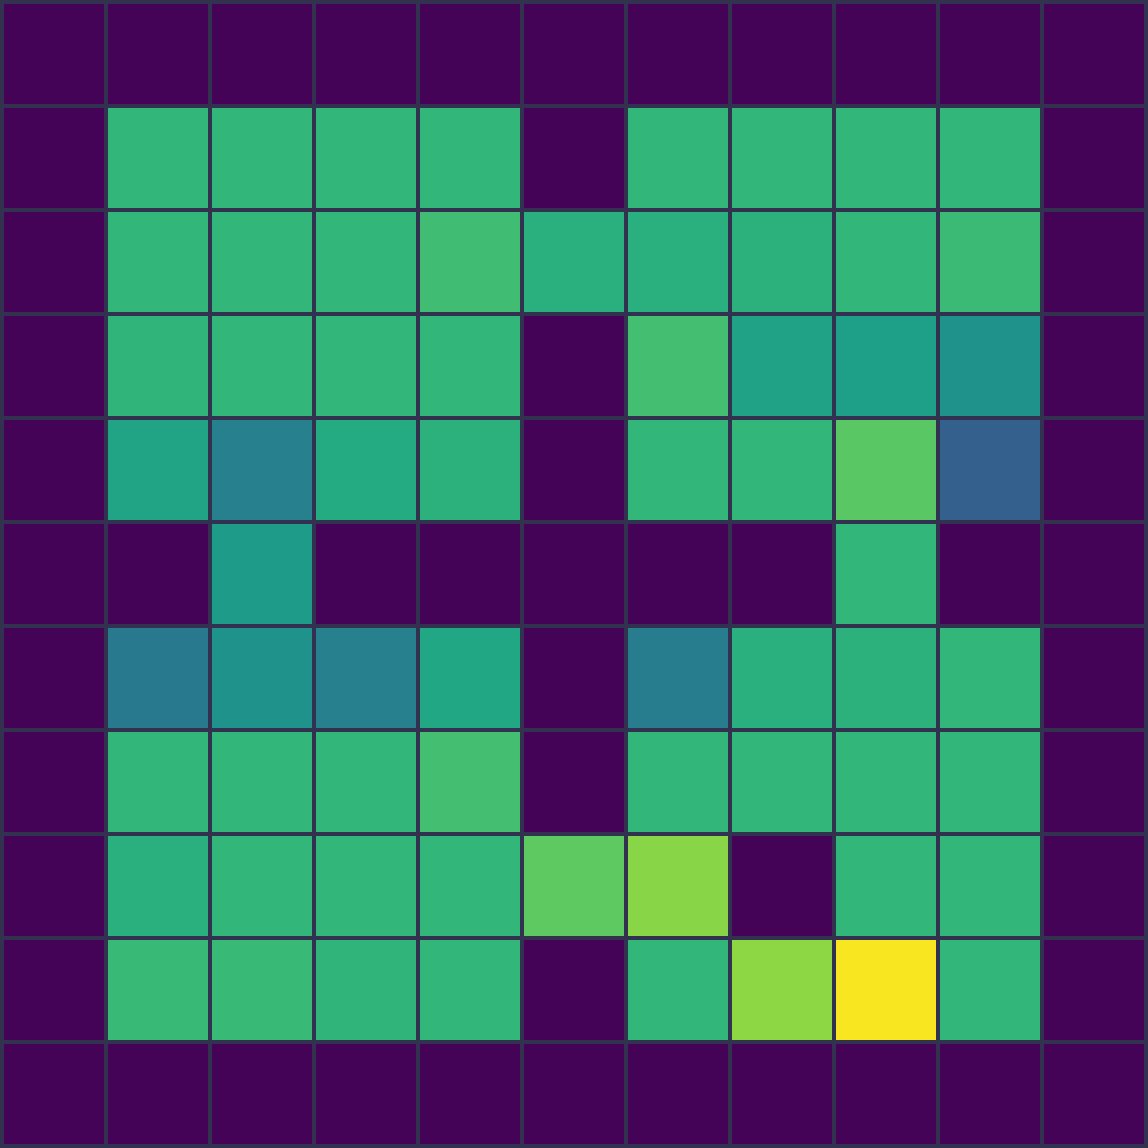
\includegraphics[width=0.09\textwidth]{image/chap04/prediction/0.png}
    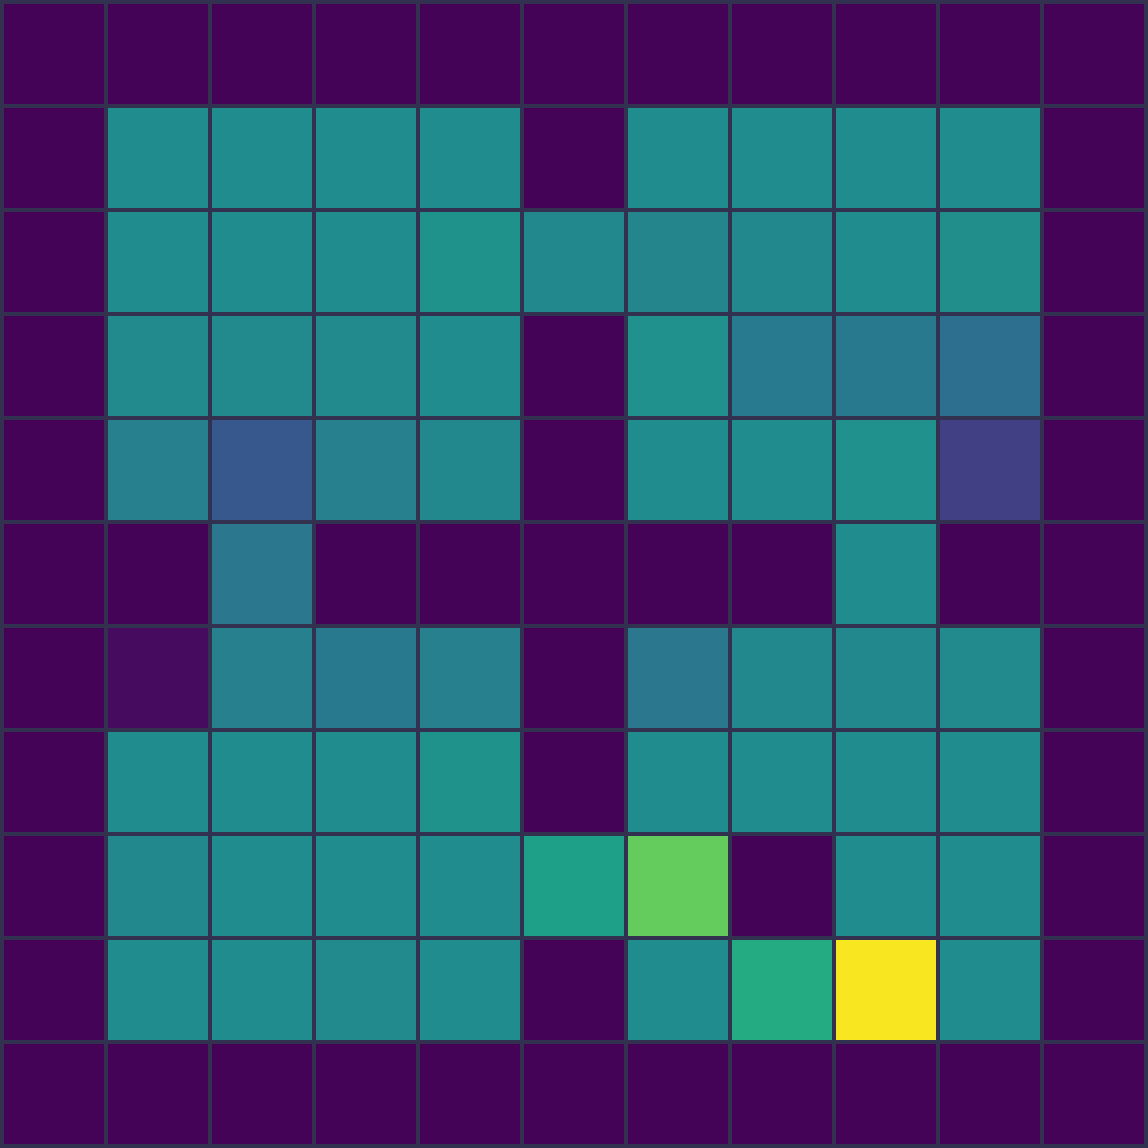
\includegraphics[width=0.09\textwidth]{image/chap04/prediction/1.png}
    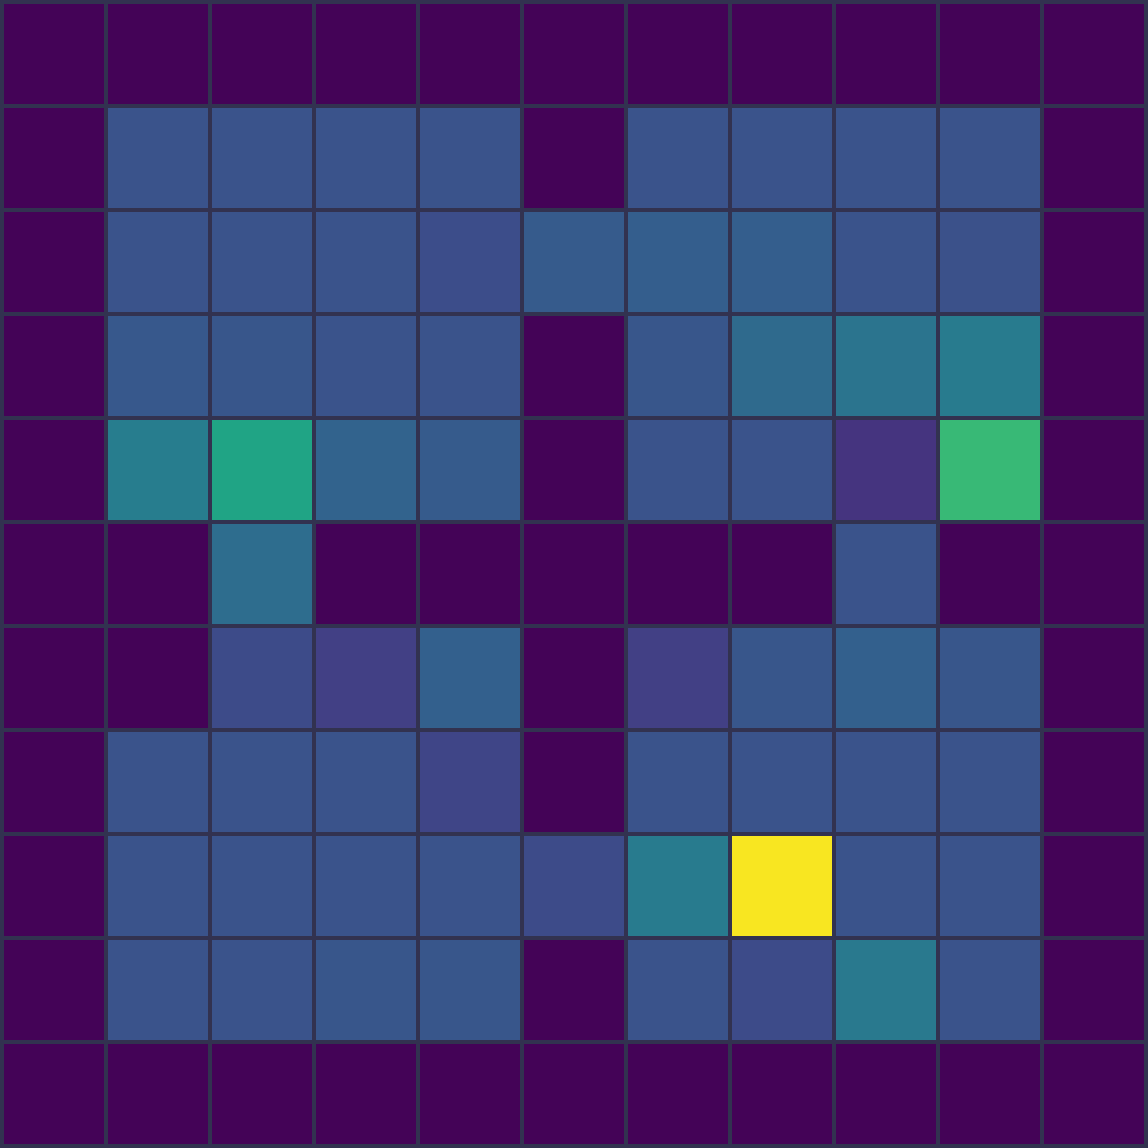
\includegraphics[width=0.09\textwidth]{image/chap04/prediction/2.png}
    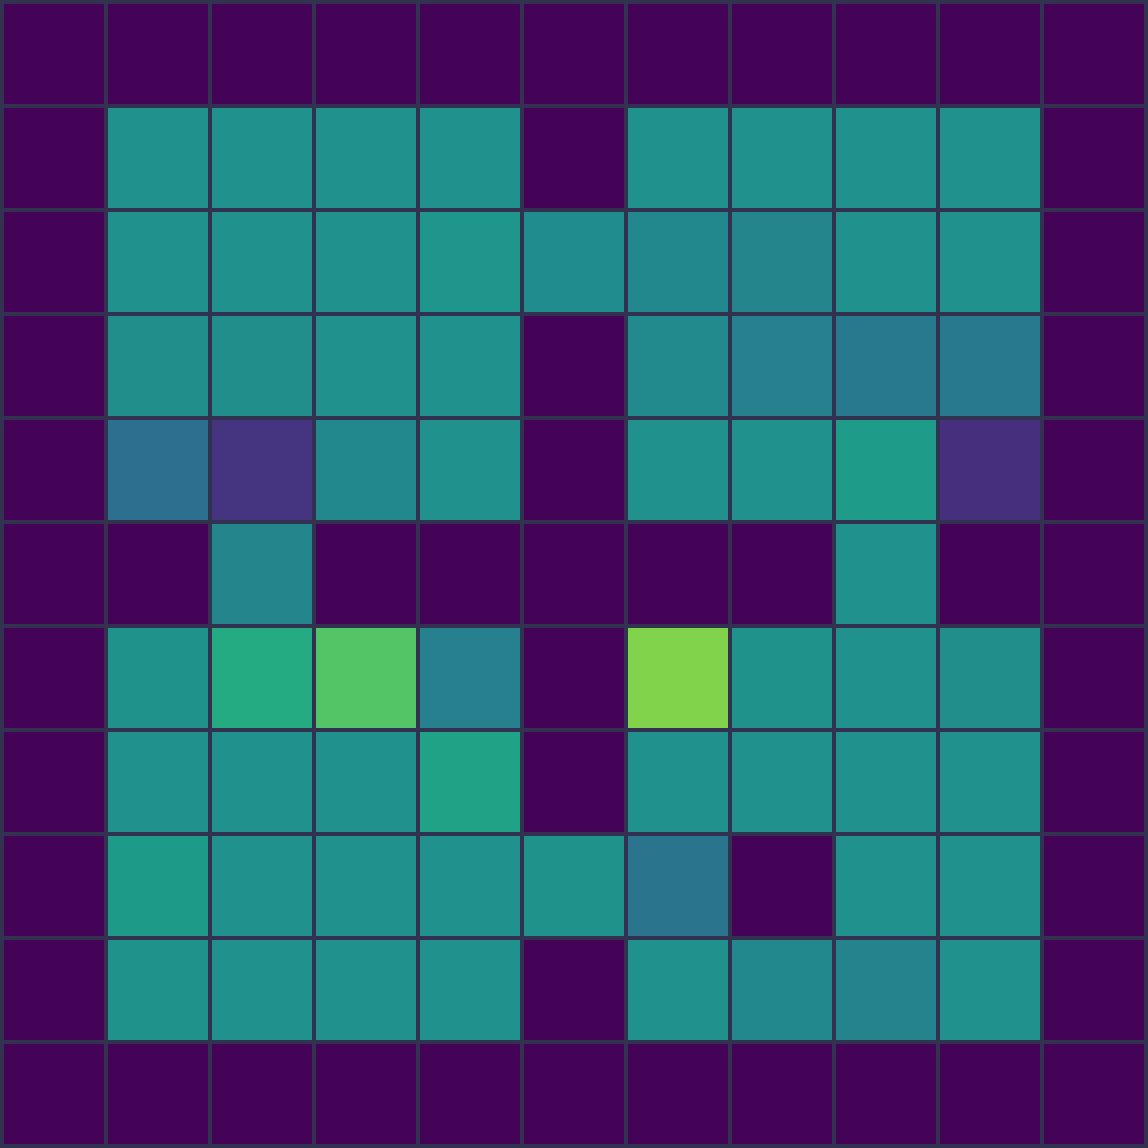
\includegraphics[width=0.09\textwidth]{image/chap04/prediction/3.png}
    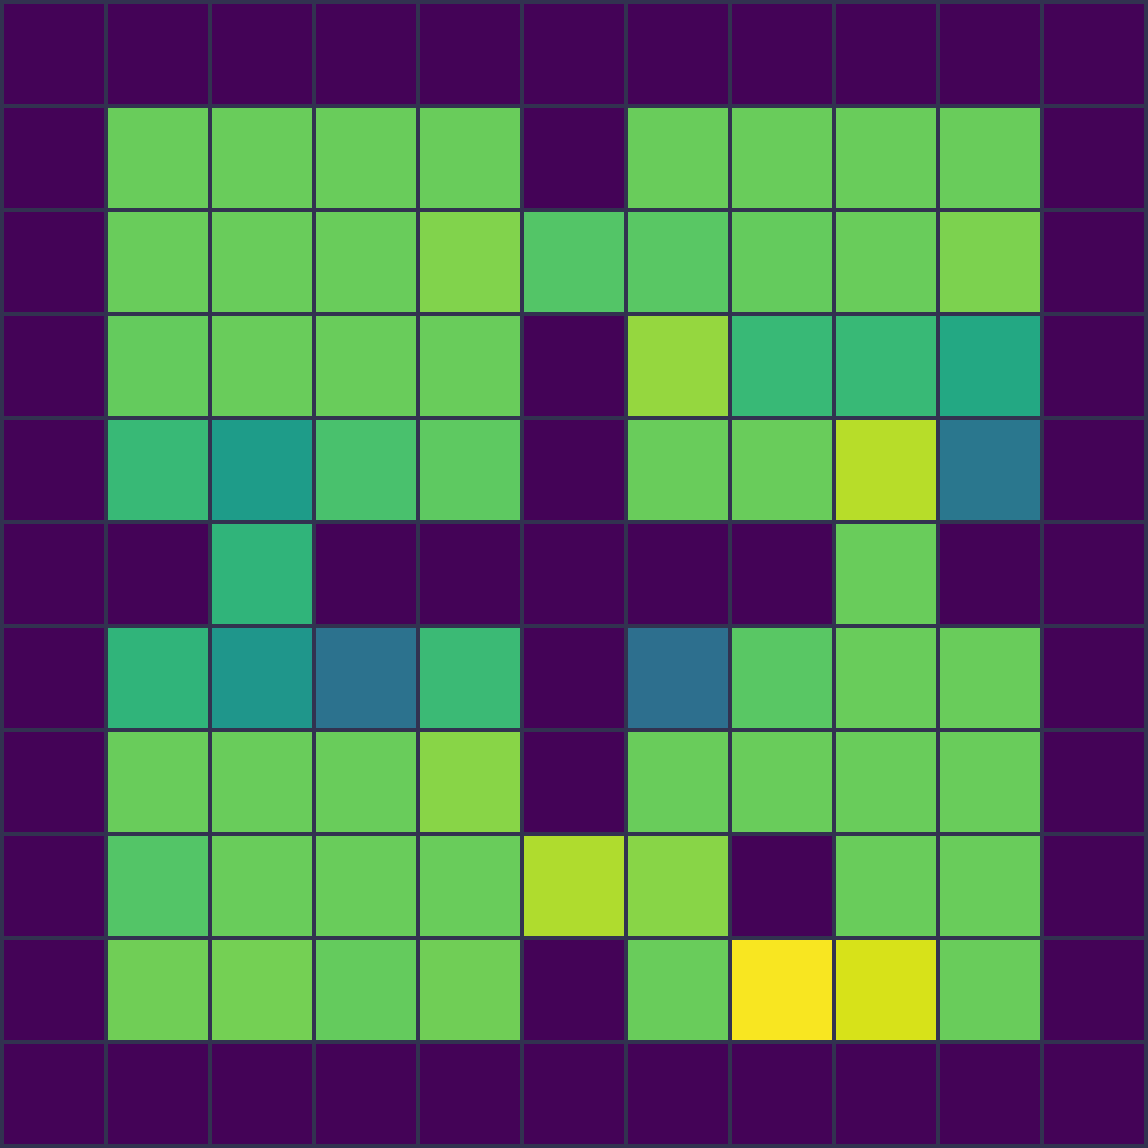
\includegraphics[width=0.09\textwidth]{image/chap04/prediction/4.png}
    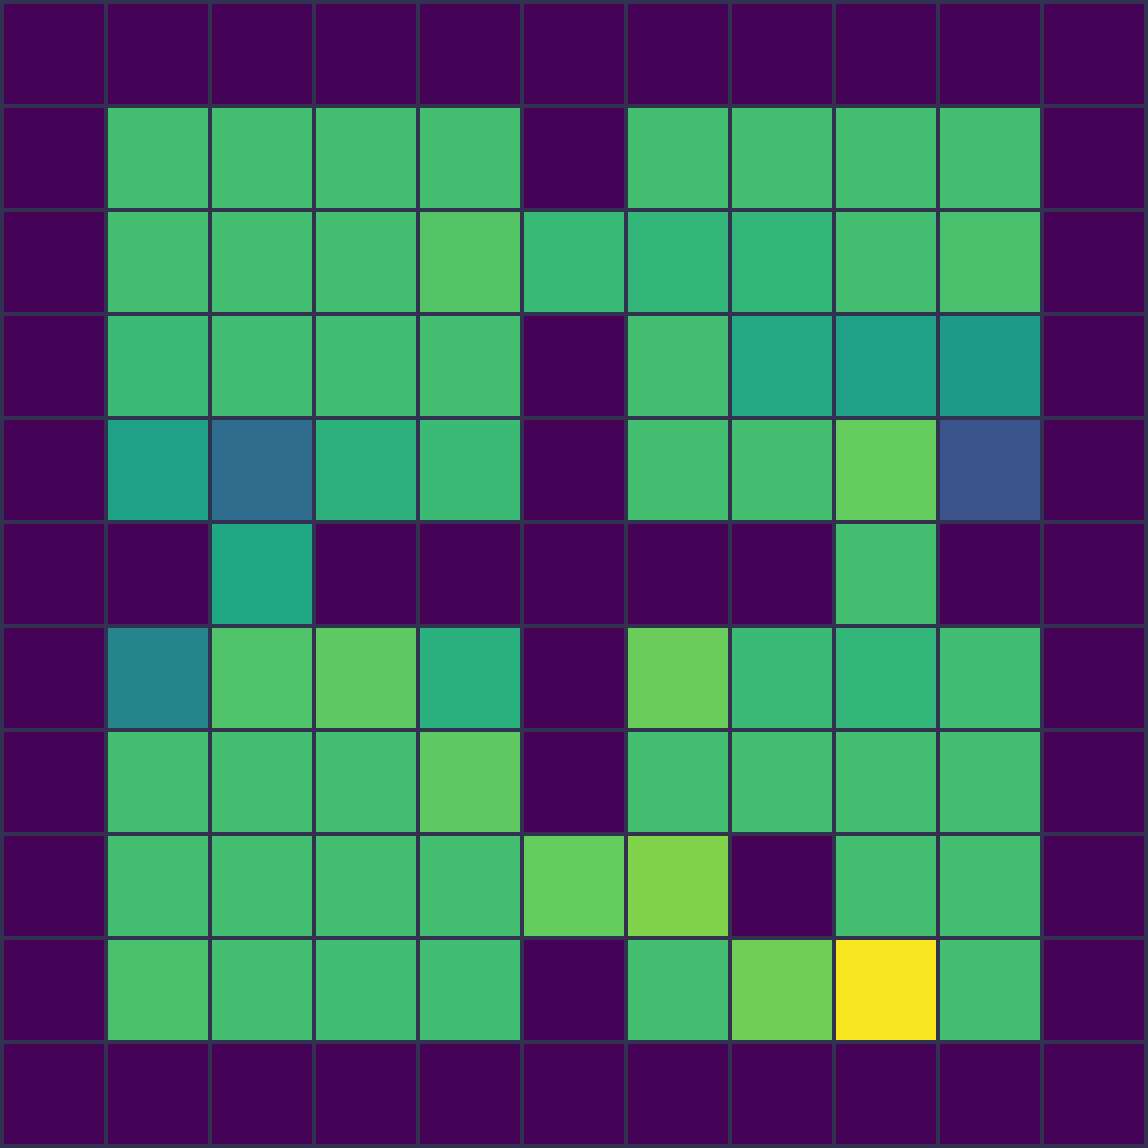
\includegraphics[width=0.09\textwidth]{image/chap04/prediction/5.png}
    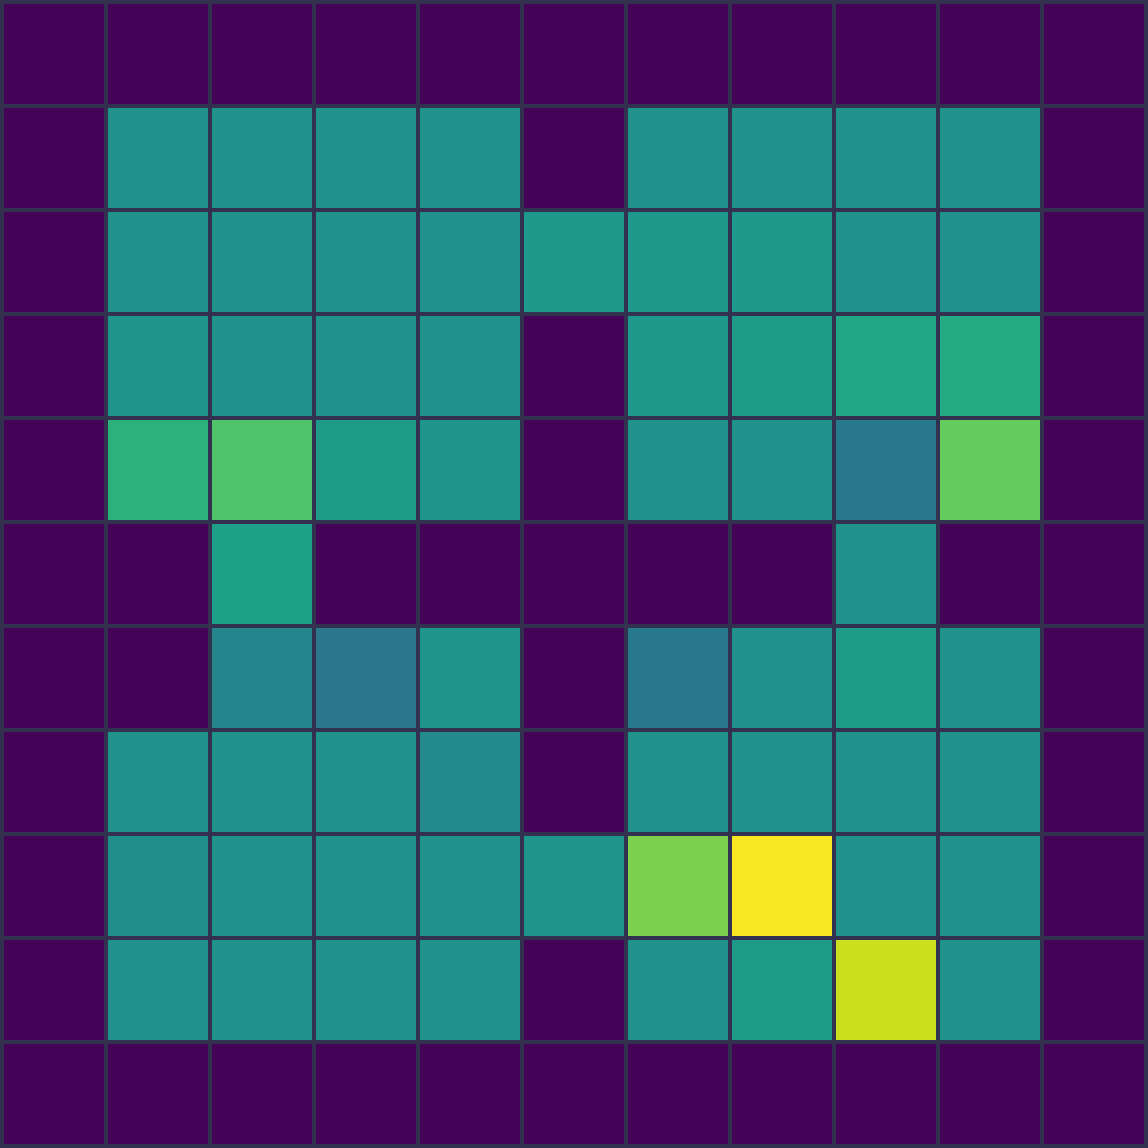
\includegraphics[width=0.09\textwidth]{image/chap04/prediction/6.png}
    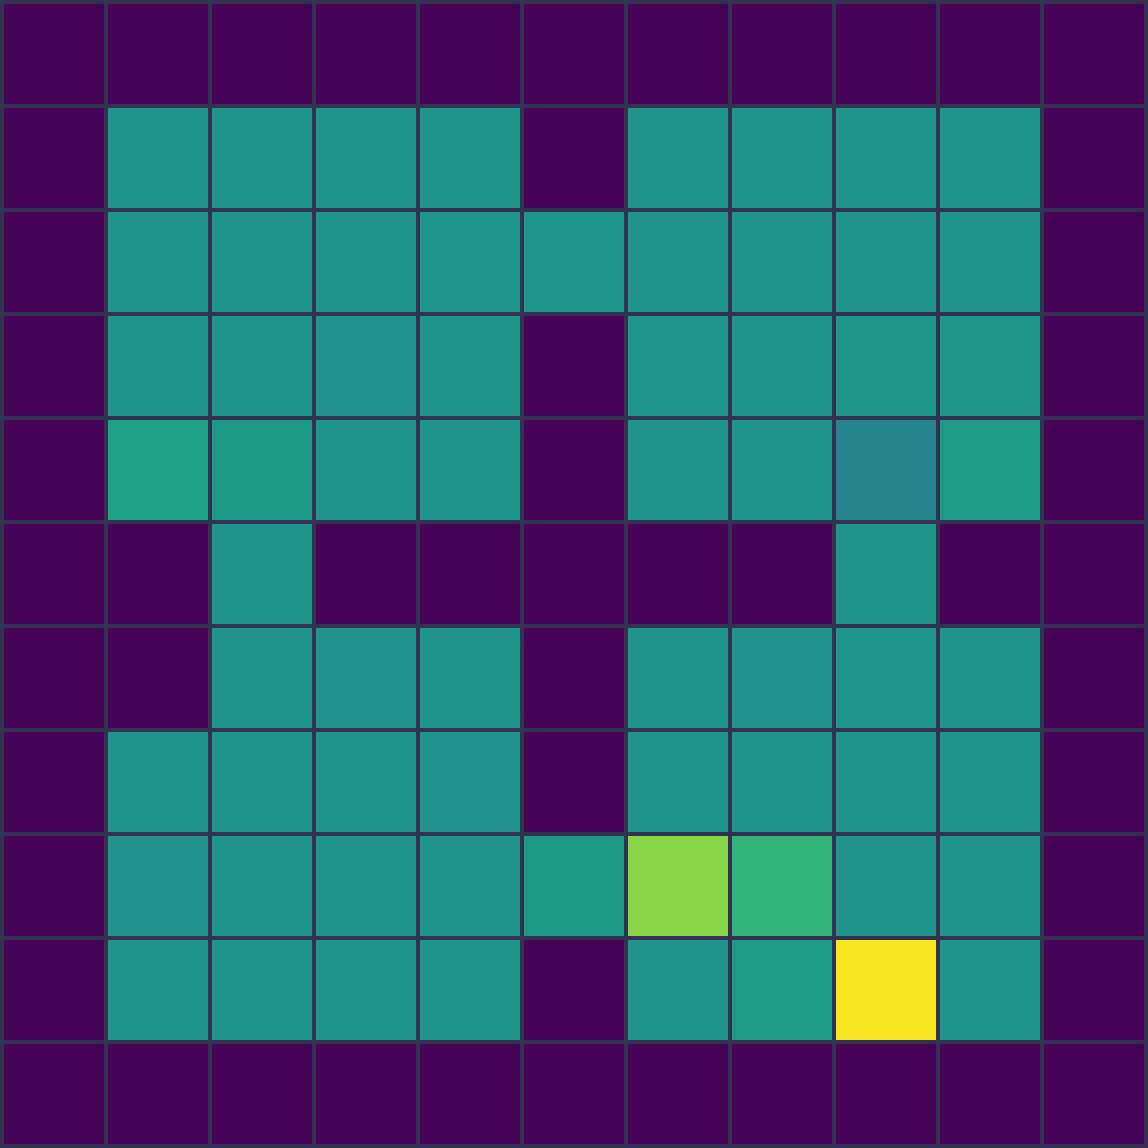
\includegraphics[width=0.09\textwidth]{image/chap04/prediction/7.png}
    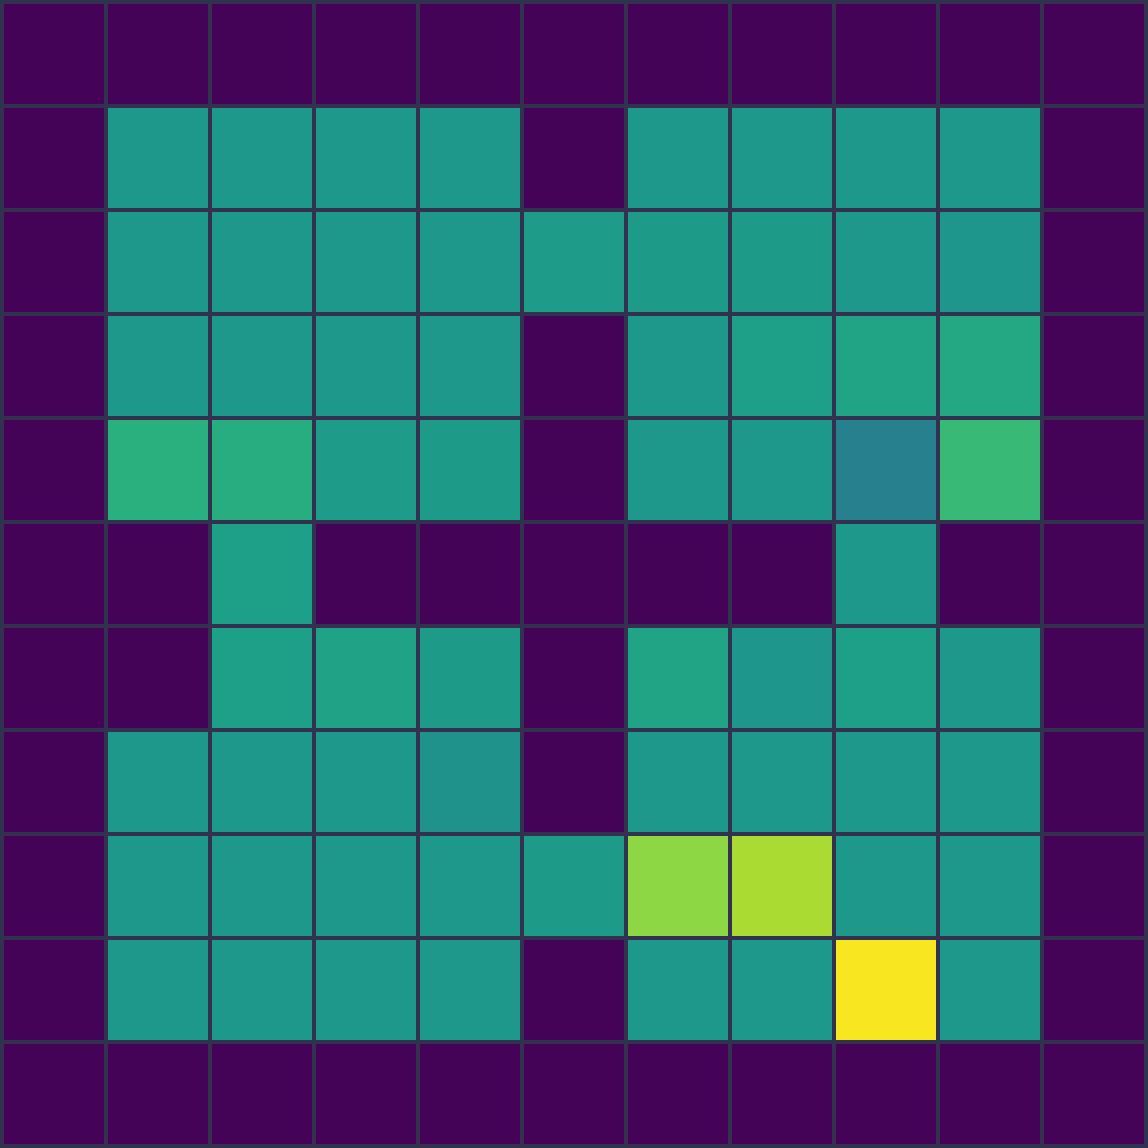
\includegraphics[width=0.09\textwidth]{image/chap04/prediction/8.png}
    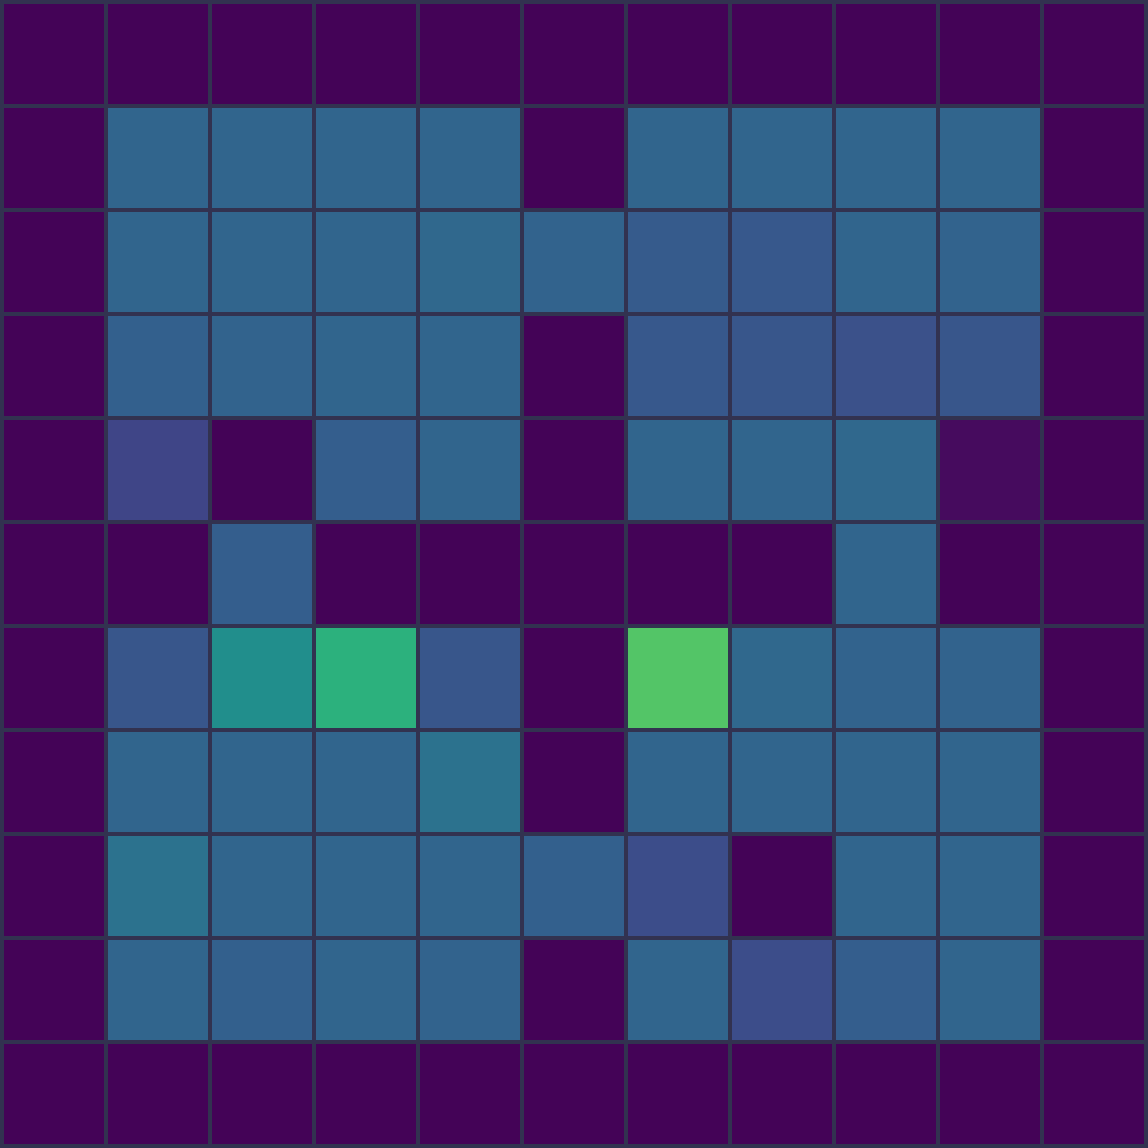
\includegraphics[width=0.09\textwidth]{image/chap04/prediction/9.png}
    \\
    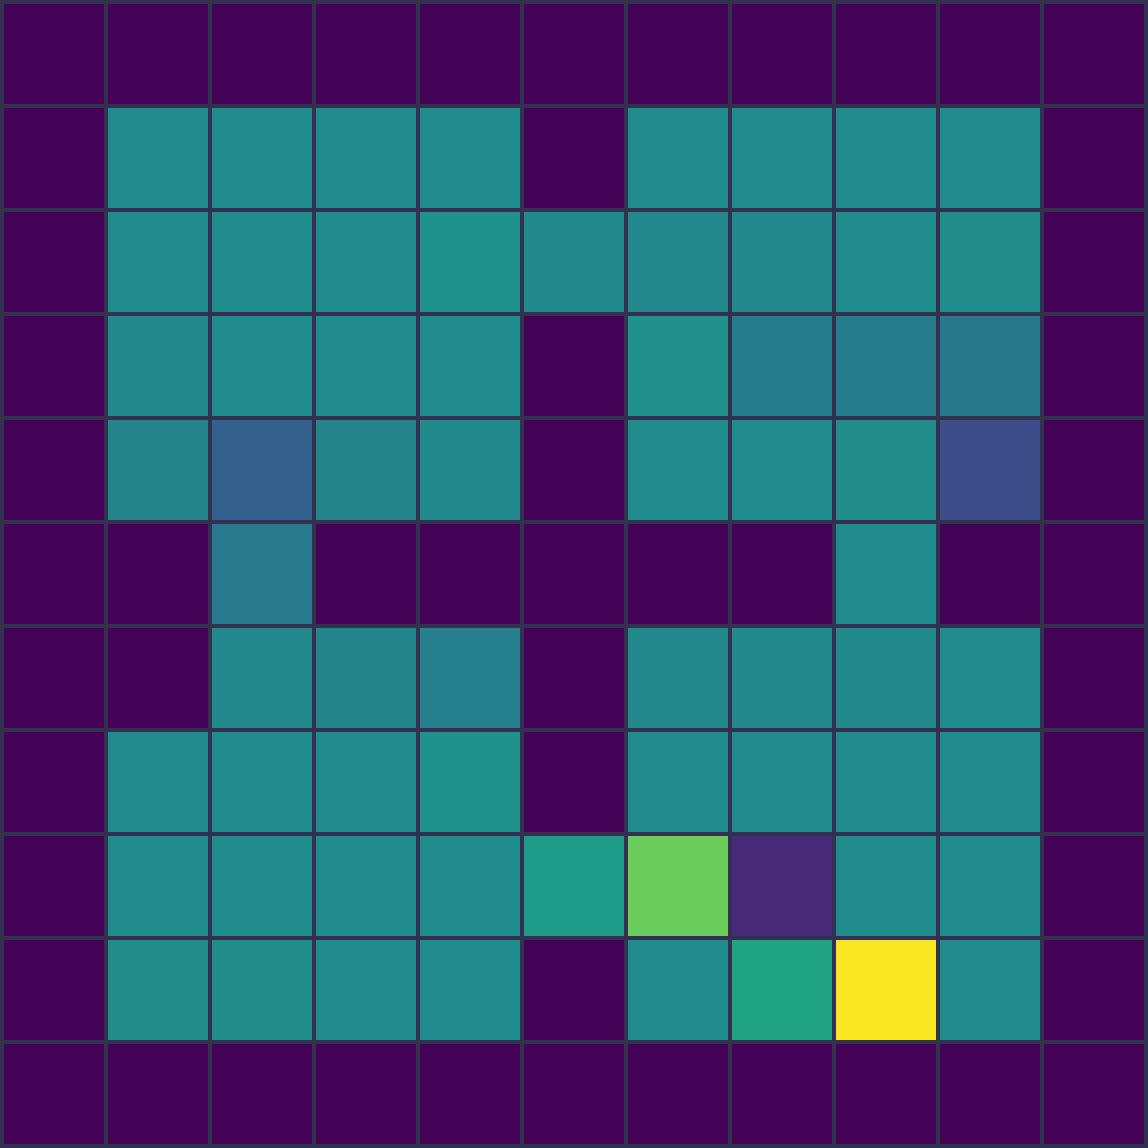
\includegraphics[width=0.09\textwidth]{image/chap04/prediction/10.png}
    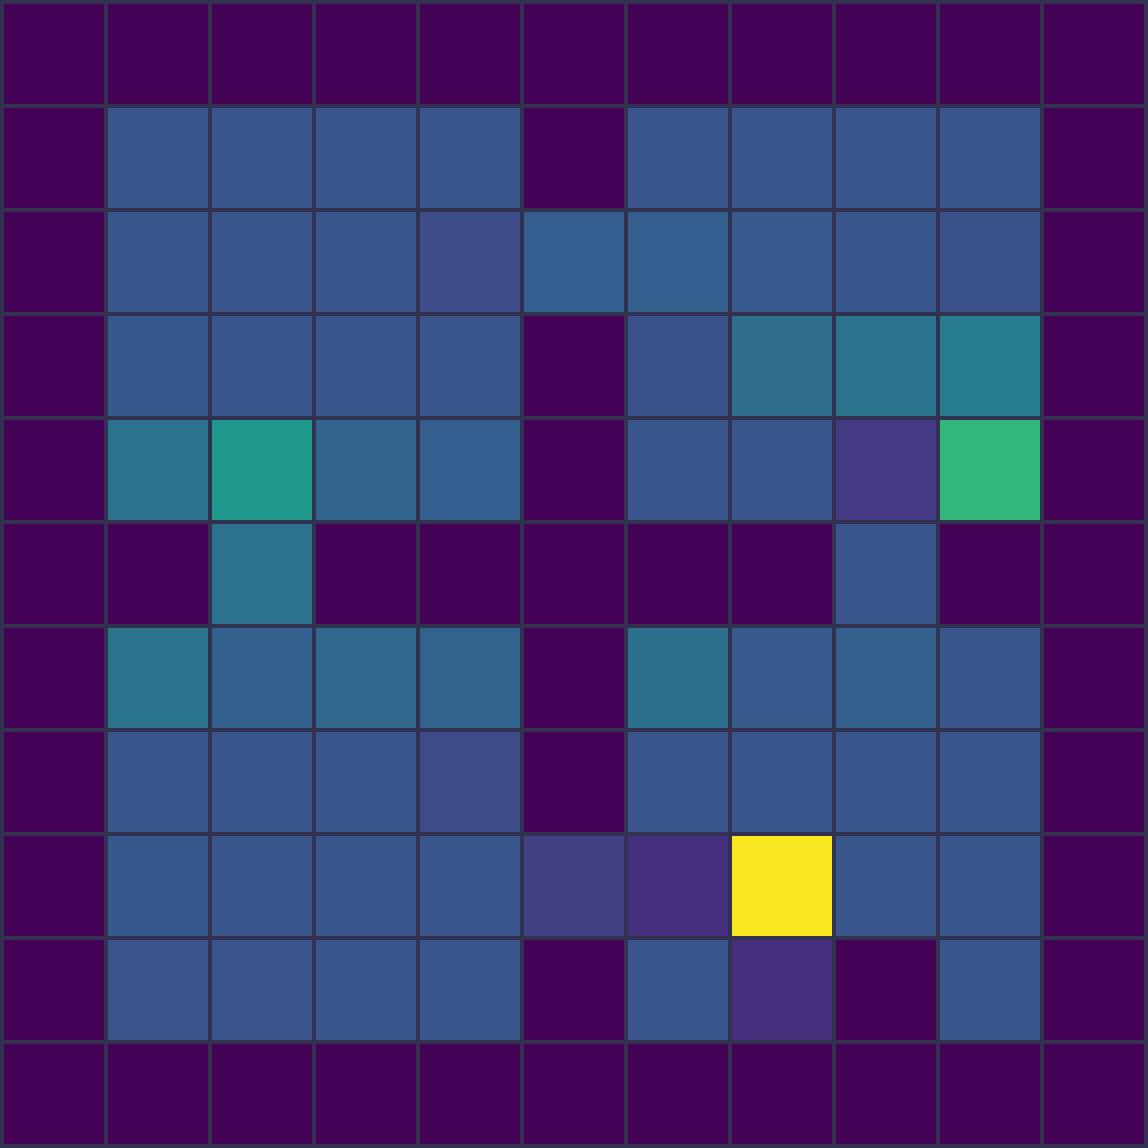
\includegraphics[width=0.09\textwidth]{image/chap04/prediction/11.png}
    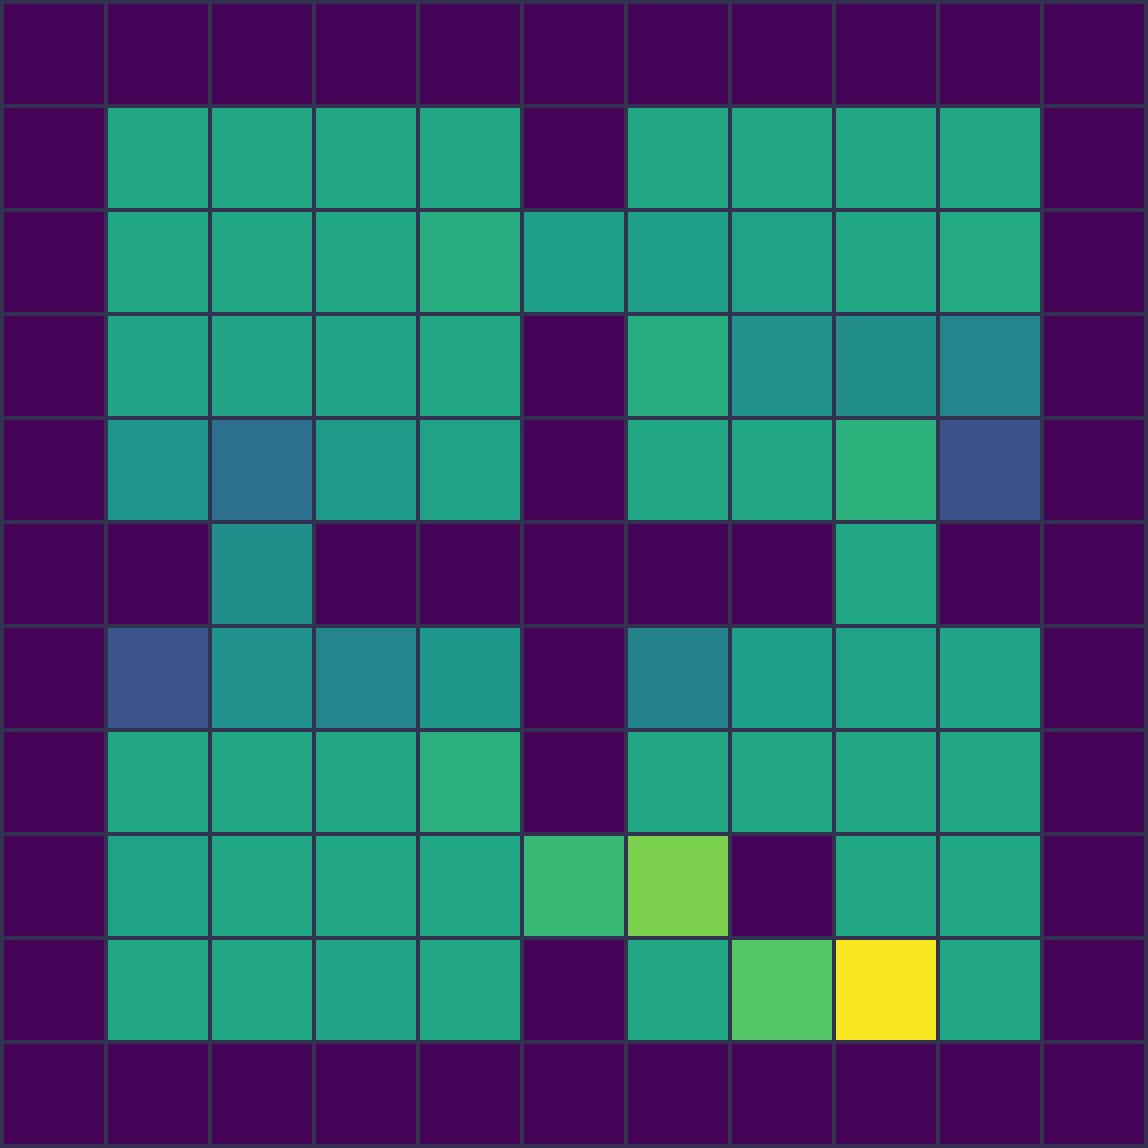
\includegraphics[width=0.09\textwidth]{image/chap04/prediction/12.png}
    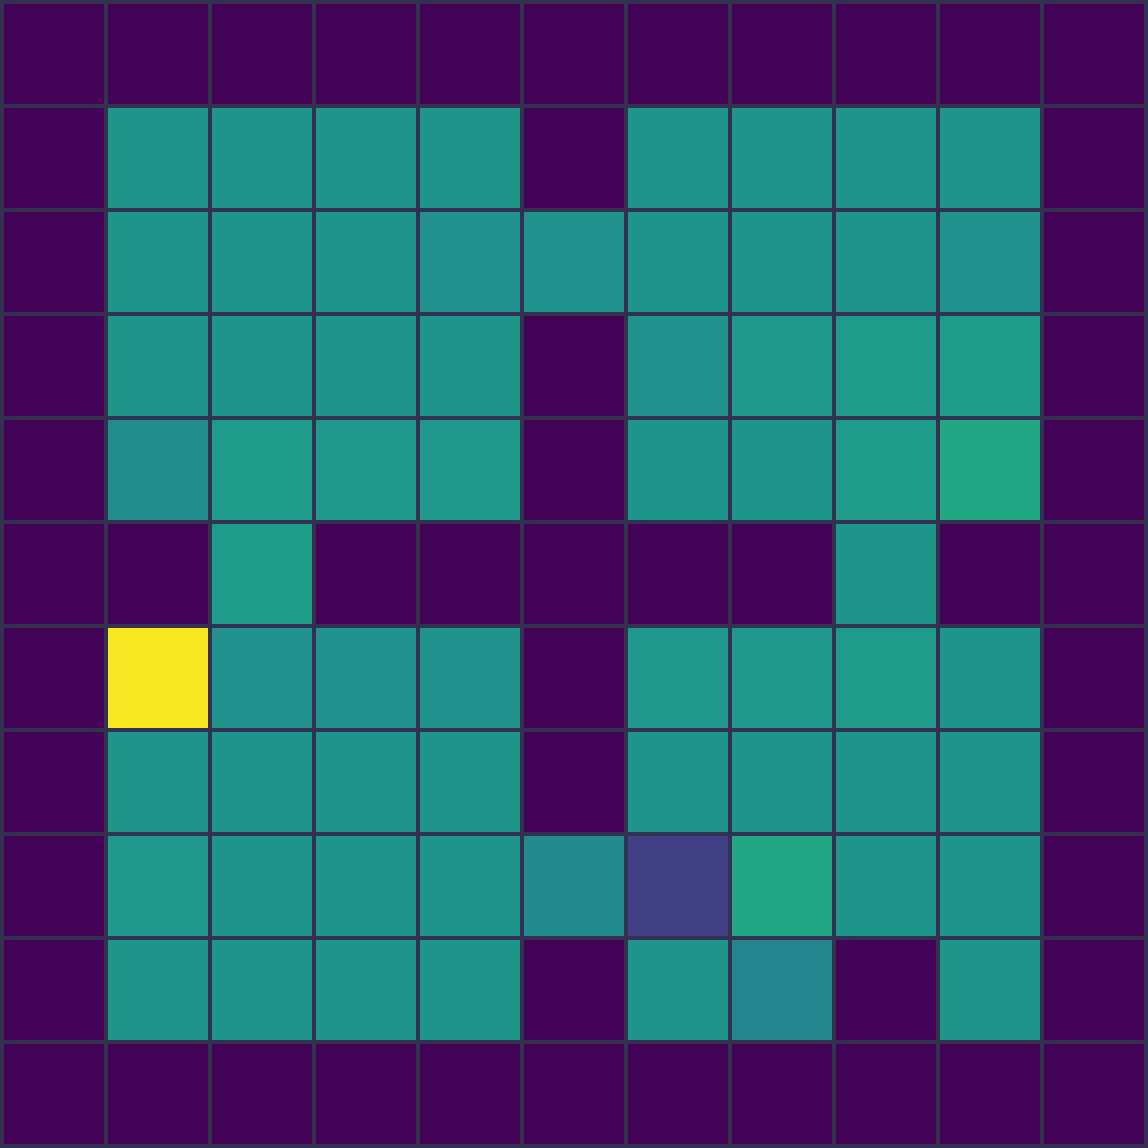
\includegraphics[width=0.09\textwidth]{image/chap04/prediction/13.png}
    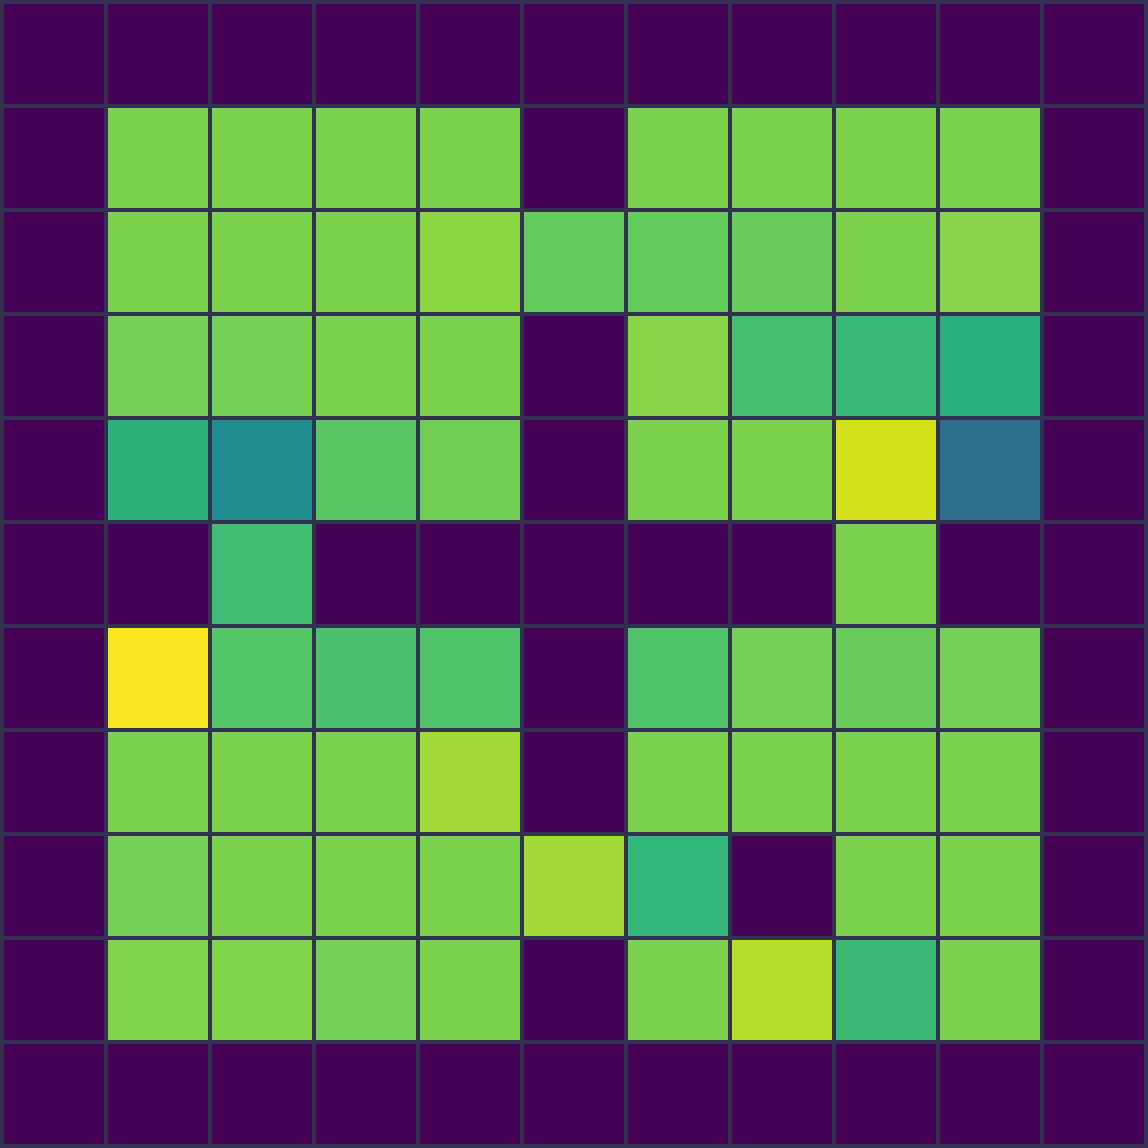
\includegraphics[width=0.09\textwidth]{image/chap04/prediction/14.png}
    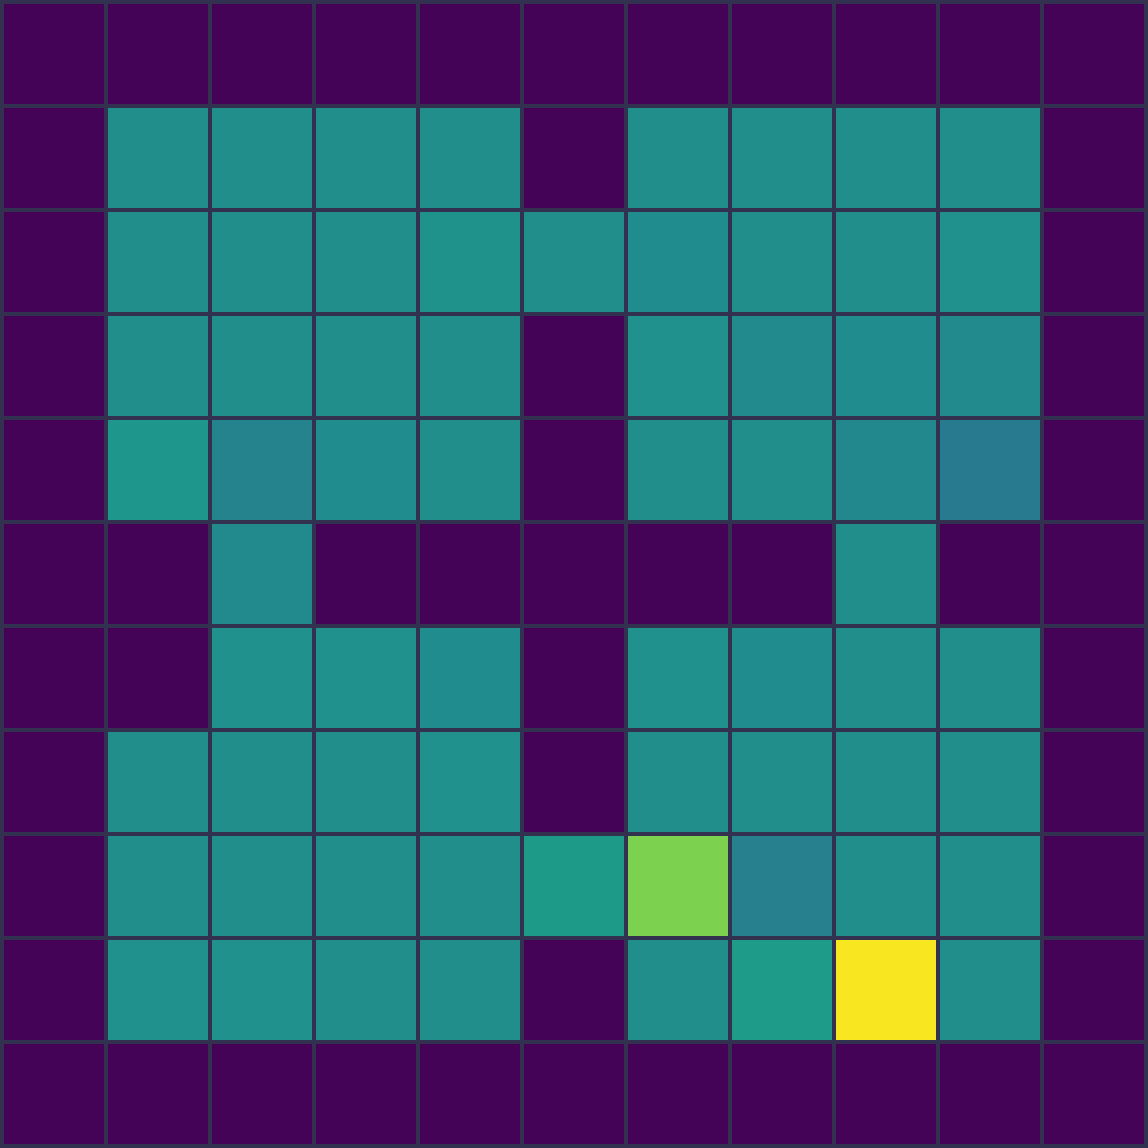
\includegraphics[width=0.09\textwidth]{image/chap04/prediction/15.png}
    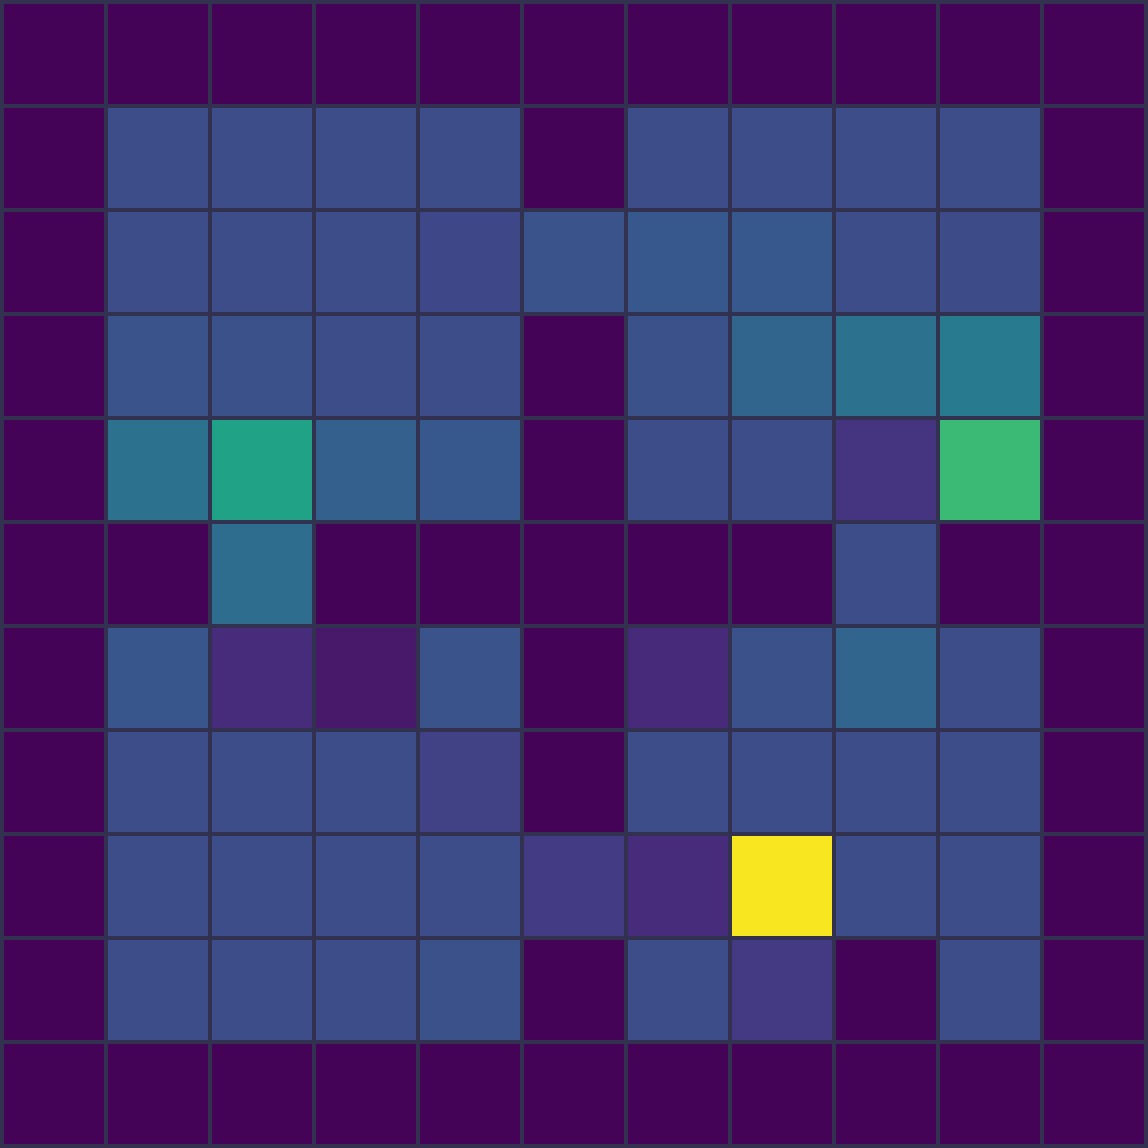
\includegraphics[width=0.09\textwidth]{image/chap04/prediction/16.png}
    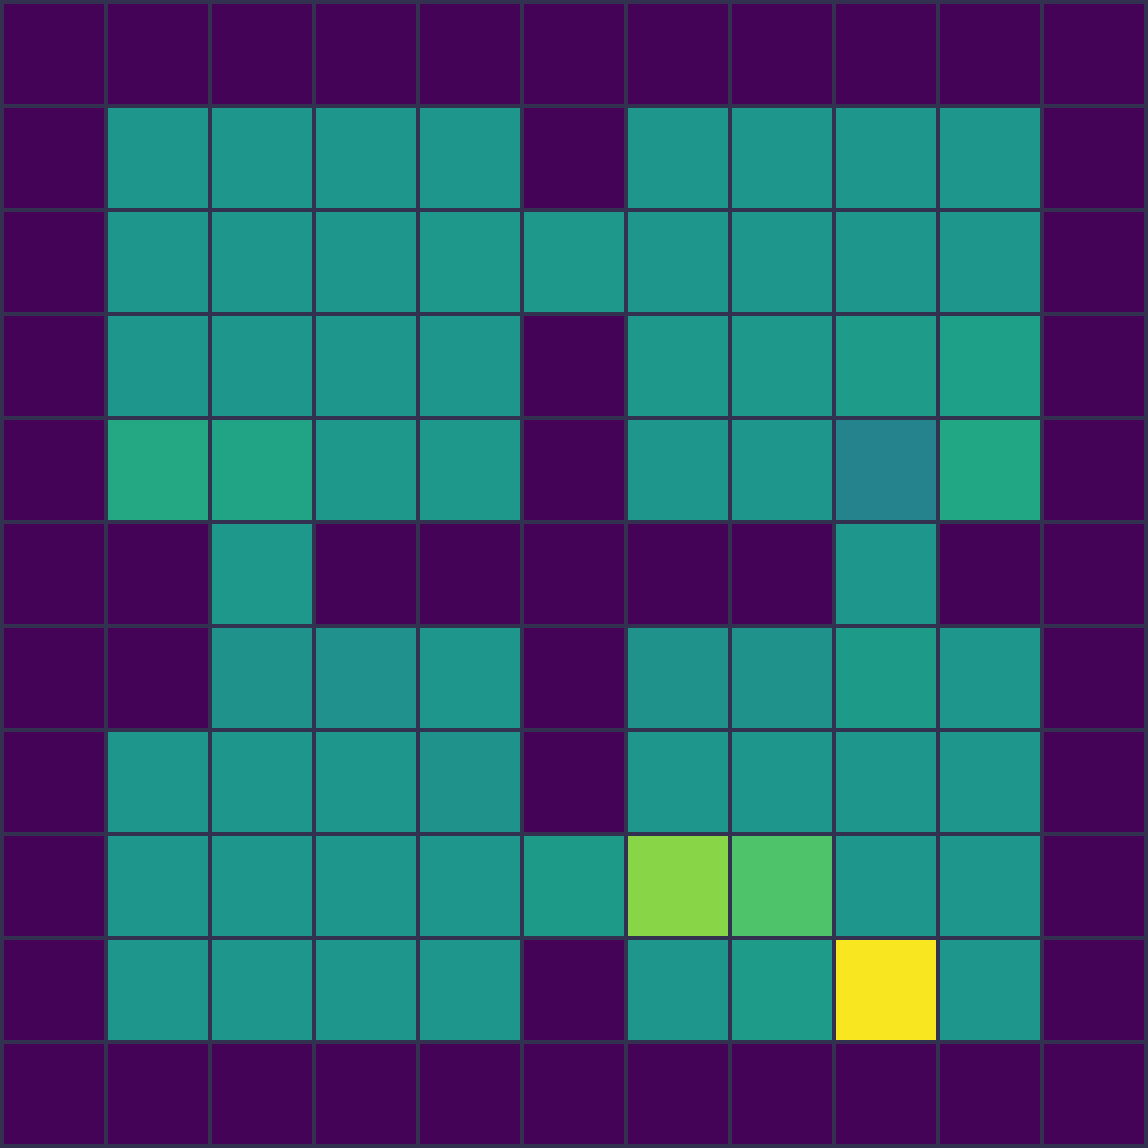
\includegraphics[width=0.09\textwidth]{image/chap04/prediction/17.png}
    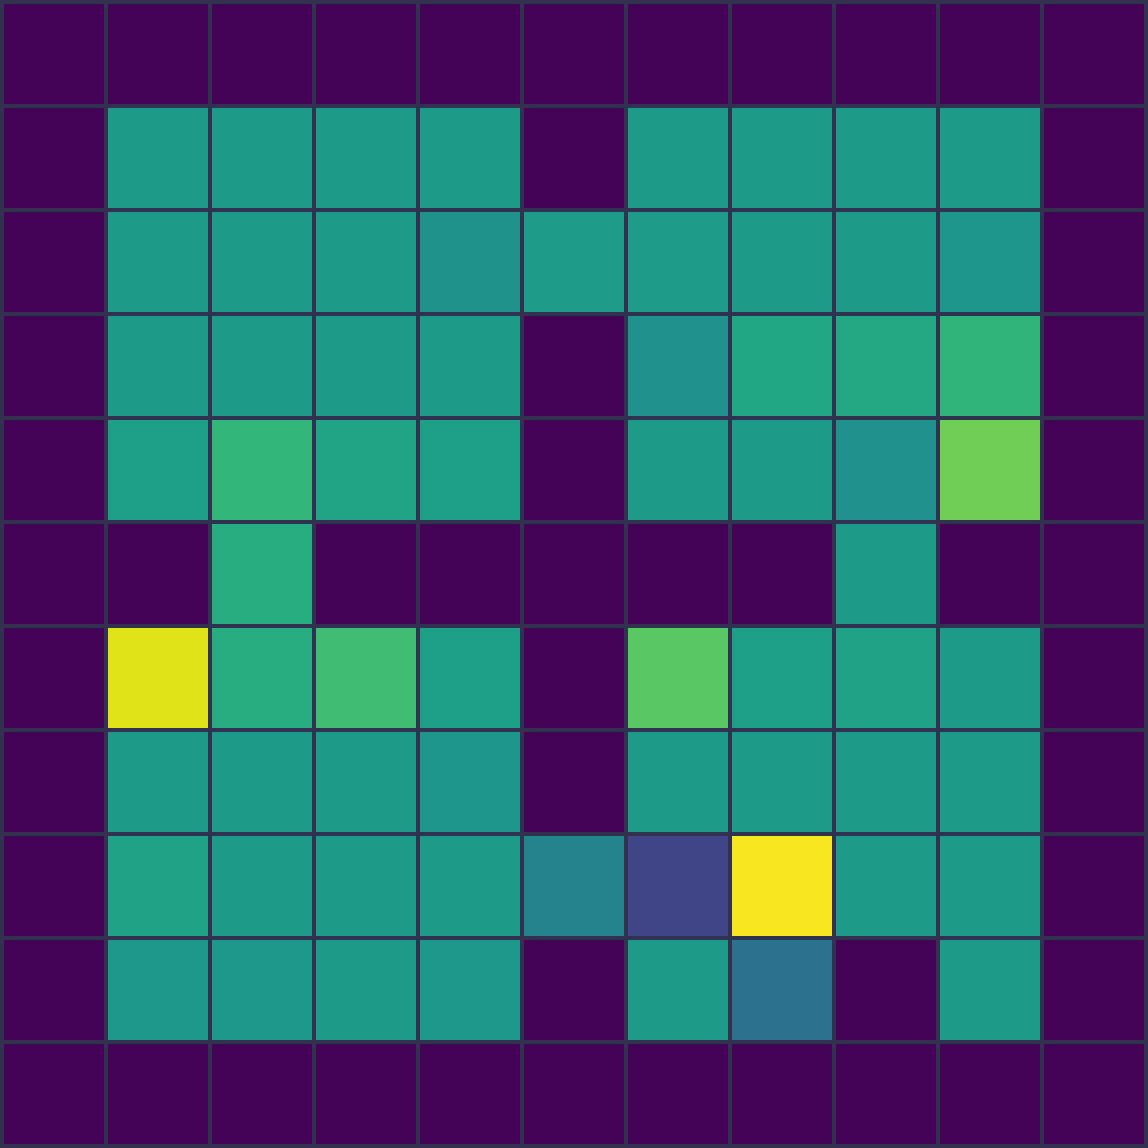
\includegraphics[width=0.09\textwidth]{image/chap04/prediction/18.png}
    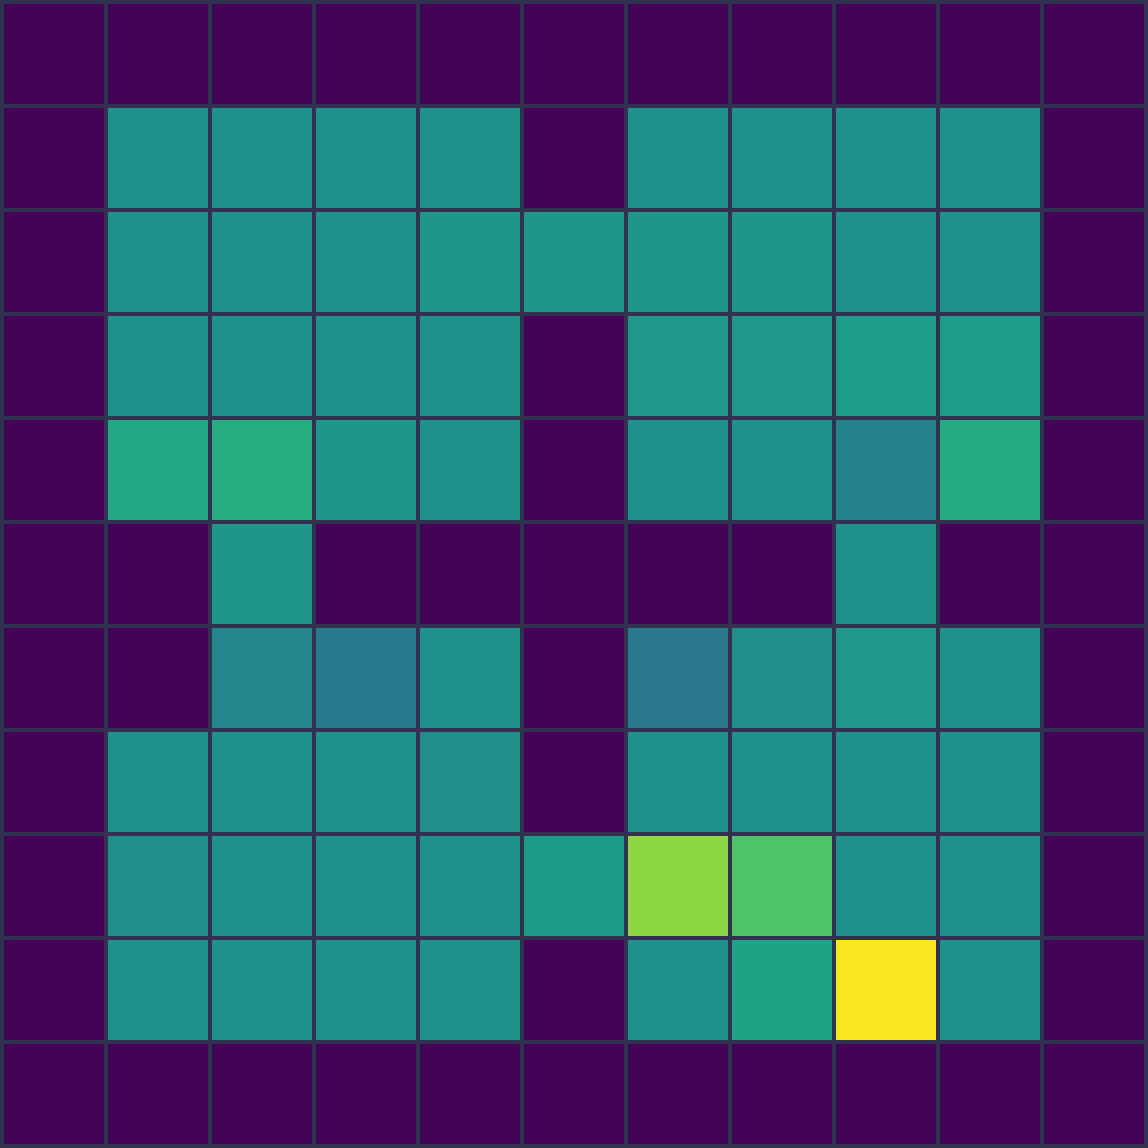
\includegraphics[width=0.09\textwidth]{image/chap04/prediction/19.png}
    \caption{预测向量}
    \label{fig:prediction}
\end{figure}

\autoref{fig:tabular}中展示了表格网格世界的实验结果,本文方法得到的策略更新方法与A2C对比。从图中可以看出来,大部分情形下,本文自适应的策略更新算法效果要好一些。以上的结果表明,在大多数训练中,本文的算法均胜过A2C。在其它环境中,可能也有同样的效果。

\begin{figure}[h!]
    \centering
    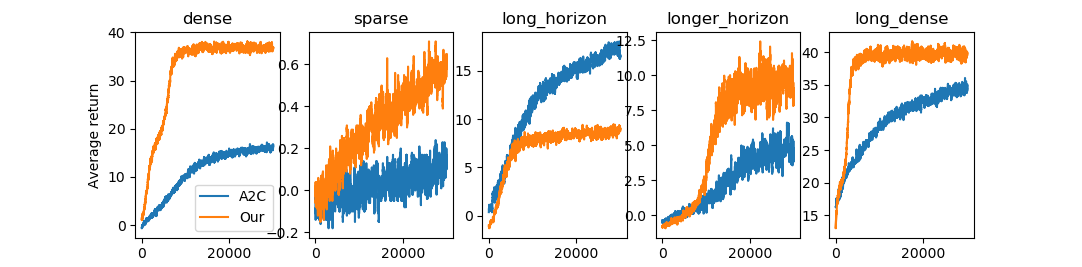
\includegraphics[width=\textwidth]{image/chap04/tabular.png}
    \caption{网格世界的实验结果}
    \label{fig:tabular}
\end{figure}
